% !TEX root = ../thesis.tex

\chapter{Grundlagen}

Zum Verständnis des Themas der Arbeit ist die Erklärung einiger Grundlagen notwendig.
Zunächst einmal werden wichtige Grundbegriffe und Datenstrukturen erläutert, wie beispielsweise Punktwolken, Meshrepräsentationen, die \textit{\ac{PCL}} oder das \textit{\ac{ROS}}.
Außerdem sind selbstverständlich die bereits bestehenden Elemente des Mikado-Projekts relevant, da diese Arbeit fundamental darauf aufbaut.
%% Vielleicht verschieben in Kapitel Vorhandene Arbeit
Weiterhin sind die Algorithmen \textit{\ac{KinFu}} beziehungsweise \textit{\ac{YAK}} wichtig, da sie das Grundgerüst oder auch das Kernelement des Themas darstellen.


\section{3D-Bilddaten}

Zur Aufnahme von 3D-Bilddaten gibt es mehrere verschiedene Möglichkeiten.
Ein LIDAR-System sendet beispielsweise mehrere Lichtstrahlen in verschiedene Richtungen, die anschließend Informationen über die Entfernung zu einem Objekt in diesem Punkt liefern.
Eine Stereokamera liefert im Gegensatz dazu zwei Bilder, die anschließend durch spezielle Software zu einem dreidimensionalen Bild zusammengesetzt werden.
Eine weitere Möglichkeit besteht darin, ein bestimmtes Muster auf die Umgebung zu projezieren, dieses dann aus einer anderen Perspektive aufzunehmen und aus der räumlichen Verzerrung des Musters die Tiefe zu errechnen.

Die so gewonnenen Informationen lassen sich durch mehrere verschiedene Datenmodelle repräsentieren.


\subsection{Tiefenbild}

Ein Tiefenbild ist eine einfache Möglichkeit, in einem zweidimensionalen Bild zusätzlich Informationen über die Entfernung der Kamera zu Objekten abzuspeichern.
Diese Technik ist unter Anderem aus der Computergrafik bekannt, wo sie beim Z-Buffering Anwendung findet \cite{strasser1974schnelle}.
Dabei werden sowohl das aufgenommene Bild, aber zusätzlich auch ein 2D-Array mit der Tiefeninformation des zugehörigen Pixels gespeichert.

So kann das originale 2D-Bild um eine dritte Dimension erweitert werden, wodurch sich beispielsweise dreidimensionale Formen modellieren oder rekonstruieren lassen \cite{arsalan2017synthesizing}.
Auch in der 3D-Fotografie finden Tiefenbilder Anwendung \cite{redert2006philips}.

\begin{figure}[ht]
	\centering
	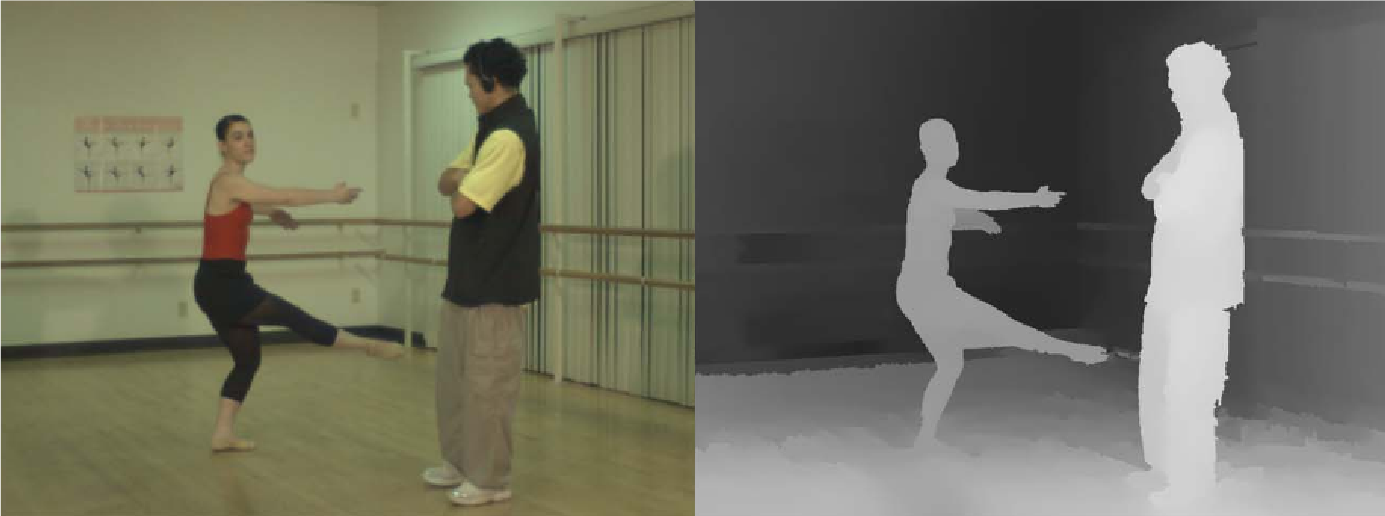
\includegraphics[width=0.66\textwidth]{images/depth_map.png}
	\caption{Depth Map eines 2D-Farbbilds. Entnommen aus \cite[S.649]{muller20103}}
	\label{fig:depth_map}
\end{figure}

Tiefenbilder haben im Vergleich zu anderen möglichen Datenmodellen den Vorteil, dass 2D-Bilder sehr einfach um zugehörige Tiefeninformationen erweitert werden können. Jedoch gibt es auch einige Nachteile, die nicht umgangen werden können:

\begin{itemize}
\item Die 3D-Daten sind ausschließlich aus der Kameraperspektive vorhanden. Um Informationen aus einer anderen Perspektive zu erhalten, muss erst aufwändig umgerechnet werden.
\item Da (in den meisten Fällen) nur ein zweidimensionales Array für die Tiefeninformation angelegt wird, können nur die Entfernungen zu den der Kamera nächsten Objekte gespeichert werden. Verdeckte, reflektierende oder durchsichtige Oberflächen können nicht gespeichert werden.
\item Das Array ist an die Auflösung der Kamera gebunden. Insbesondere bei großer Entfernung zu Objekten werden diese aufgrund des Bildwinkels sehr schlecht abgetastet, was später zu Aliasing-Effekten führen kann.
\item Die Bittiefe der Werte im Array kann - je nach gewünschter Auflösung - zu niedrig sein, bzw. muss erhöht werden. Eine typische Farbtiefe eines Grauwertbilds von 8 Bit repräsentiert beispielsweise nur $2^8 = 256$ Stufen - was schnell zu wenig wird. Insbesondere bei hoher notwendiger Auflösung im nahen Bereich, aber gleichzeitig vorhandenen weit entfernten Objekten kann dies zum Problem werden.
\end{itemize}


\subsection{Voxel Grid}

In einem Voxel Grid wird ein dreidimensionales Raster, bestehend aus den sogenannten Voxeln, angelegt.
Die Tiefeninformation wird dann in den Voxeln gespeichert: Ist ein Voxel teil eines Elements, wird er gefüllt, andernfalls nicht.


\subsection{Punktwolken}

Ein weiteres häufig verwendetes Datenmodell ist eine Punktwolke.
Als Punktwolke bezeichnet man eine Menge $M \subset \mathbb{R}^3$ von Punkten im (mindestens) dreidimensionalen Raum.
Zusätzlich zur räumlichen Information können auch noch weitere Daten pro Punkt gespeichert sein, wie RGB-Werte, Genauigkeit oder Objektklasse (falls schon eine Segmentierung vorgenommen wurde).
Dadurch gilt:
$$M = \begin{pmatrix}
p_x^1 & p_y^1 & p_z^1 & \cdots\\
p_x^2 & p_y^2 & p_z^2 & \cdots\\
p_x^3 & p_y^3 & p_z^3 & \cdots\\
\vdots & \vdots & \vdots & \ddots
\end{pmatrix}$$

Die Nutzung von Punktwolken bringt im Vergleich zu anderen 3D-Datenmodellen einige Vorteile.


\section{Meshrepräsentationen}


\section{Point Cloud Library}


\section{Robot Operating System}
